\section{Appendix A}
\label{sec:appendix-a}

\subsection{Git Internals}


  \code{Git} - is a simple key-value data store that stores 3 main types of Objects: \code{blob}, \code{tree}, \code{commit}, and one additional: \code{tag}.
  Git stores content in a manner similar to a UNIX filesystem,
  but a bit simplified.
  All the content is stored as tree and blob objects,
  with trees corresponding to UNIX directory entries and blobs corresponding more or less to inodes or file contents.

  Conceptually, the data that Git is storing looks something like this::\\

  \begin{figure}[H]
    \begin{center}
      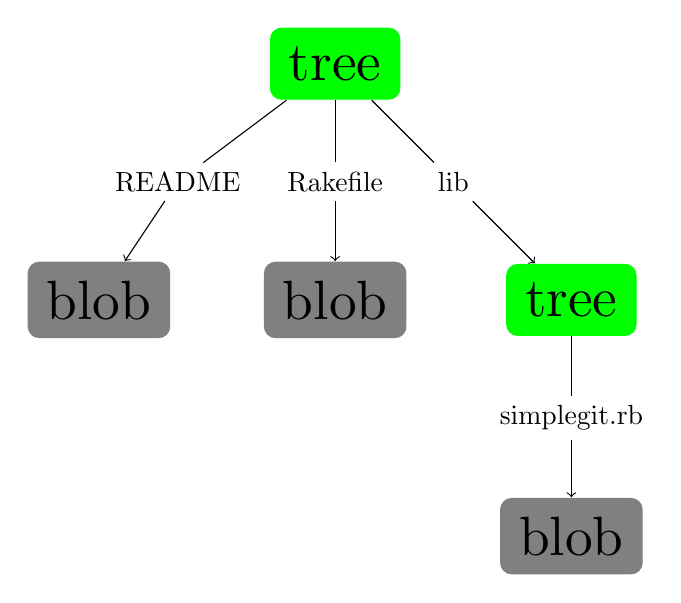
\begin{tikzpicture}
        \node[rectangle,rounded corners, draw=green, fill=green, scale=2] (tree) at(0,0){tree};
        \node[rectangle,rounded corners, draw=gray, fill=gray, scale=2] (Rakefile-blob) at(0,-3){blob};
        \node[rectangle,rounded corners, draw=gray, fill=gray, scale=2] (README-blob) at(-3,-3){blob};
        \node[rectangle,rounded corners, draw=green, fill=green, scale=2] (lib-tree) at(3,-3){tree};
        \node[rectangle,rounded corners, draw=gray, fill=gray, scale=2] (simplegit-blob) at(3,-6){blob};

        \node[rectangle,rounded corners, draw=white, fill=white] (Rakefile) at(0,-1.5){Rakefile};
        \node[rectangle,rounded corners, draw=white, fill=white] (README) at(-2,-1.5){README};
        \node[rectangle,rounded corners, draw=white, fill=white] (lib) at(1.5,-1.5){lib};
        \node[rectangle,rounded corners, draw=white, fill=white] (simplegit) at(3,-4.5){simplegit.rb};

        \draw (tree) -- (Rakefile);
        \draw [->] (Rakefile) -- (Rakefile-blob);

        \draw (tree) to (README);
        \draw [->] (README) to (README-blob);

        \draw (tree) -- (lib);
        \draw [->] (lib) -- (lib-tree);

        \draw (lib-tree) -- (simplegit);
        \draw [->] (simplegit) -- (simplegit-blob);


      \end{tikzpicture}
    \end{center}
    \caption{Simple version of the Git data model}
    \label{fig:git-tree-sample}
  \end{figure}

  Blobs store content without file names and trees store filenames and also allows to store a group of files together.
  Top level trees represent the different snapshots of a project that you want to track.

  Commit objects point to that top level trees(snapshots)
  and store information about who saved the snapshots, when they were saved, or why they were saved.

  To order snapshots Commit object also points to parent(previous) commit if any.

  So snapshots could be reached and tracked via commit objects.

  \begin{figure}[H]
    \begin{center}
      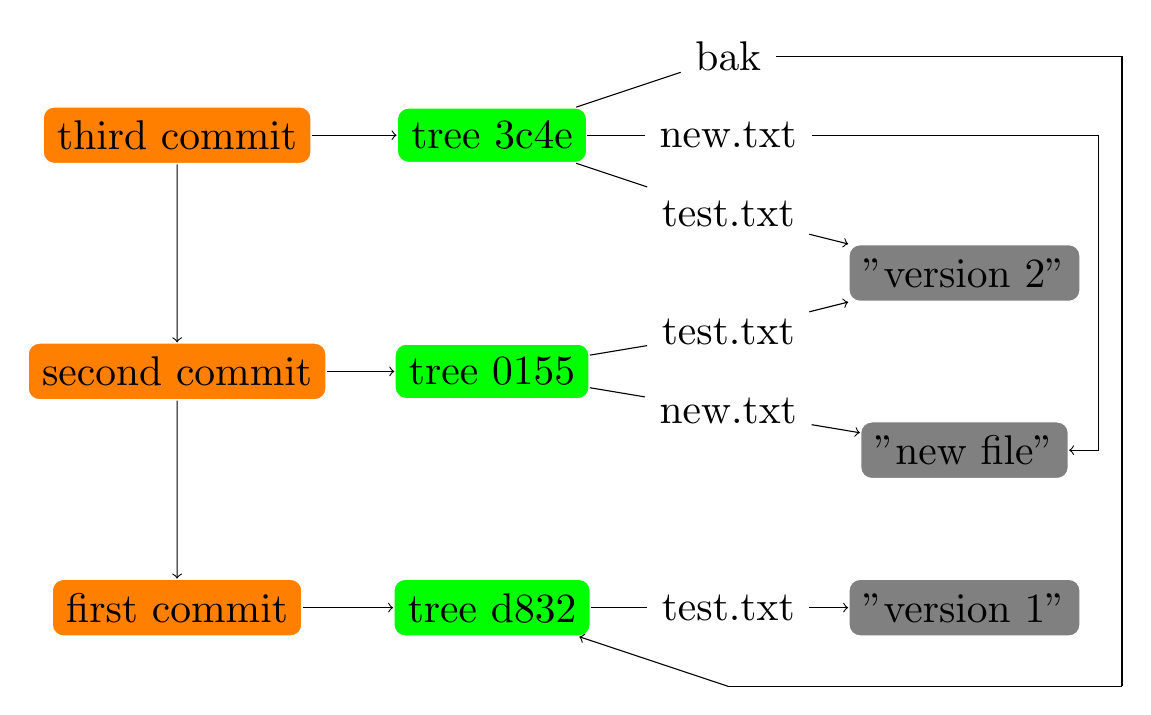
\begin{tikzpicture}
        \node[rectangle,rounded corners, draw=white, fill=orange, scale=1.5] (3-commit) at(0,0){third commit};
        \node[rectangle,rounded corners, draw=white, fill=orange, scale=1.5] (2-commit) at(0,-3){second commit};
        \node[rectangle,rounded corners, draw=white, fill=orange, scale=1.5] (1-commit) at(0,-6){first commit};
        \draw [->] (3-commit) -- (2-commit);
        \draw [->] (2-commit) -- (1-commit);

        \node[rectangle,rounded corners, draw=white, fill=green, scale=1.5] (3-tree) at(4,0){tree 3c4e};
        \draw [->] (3-commit) -- (3-tree);

        \node[rectangle,rounded corners, draw=white, fill=green, scale=1.5] (2-tree) at(4,-3){tree 0155};
        \draw [->] (2-commit) -- (2-tree);

        \node[rectangle,rounded corners, draw=white, fill=green, scale=1.5] (1-tree) at(4,-6){tree d832};
        \draw [->] (1-commit) -- (1-tree);

        \node[rectangle,rounded corners, draw=white, fill=white, scale=1.5] (3-bak) at(7,1){bak};
        \node[rectangle,rounded corners, draw=white, fill=white, scale=1.5] (3-new) at(7,0){new.txt};
        \node[rectangle,rounded corners, draw=white, fill=white, scale=1.5] (3-test) at(7,-1){test.txt};

        \node[rectangle,rounded corners, draw=white, fill=white, scale=1.5] (2-test) at(7,-2.5){test.txt};
        \node[rectangle,rounded corners, draw=white, fill=white, scale=1.5] (2-new) at(7,-3.5){new.txt};

        \node[rectangle,rounded corners, draw=white, fill=white, scale=1.5] (1-test) at(7,-6){test.txt};

        \draw (3-tree) -- (3-bak);
        \draw (3-tree) -- (3-new);
        \draw (3-tree) -- (3-test);

        \draw (2-tree) -- (2-test);
        \draw (2-tree) -- (2-new);

        \draw (1-tree) -- (1-test);

        \node[rectangle,rounded corners, draw=white, fill=gray, scale=1.5] (version-2) at(10,-1.75){"version 2"};
        \node[rectangle,rounded corners, draw=white, fill=gray, scale=1.5] (new-file) at(10,-4){"new file"};
        \node[rectangle,rounded corners, draw=white, fill=gray, scale=1.5] (version-1) at(10,-6){"version 1"};

        \draw [->] (1-test) -- (version-1);
        \draw [->] (2-new) -- (new-file);
        \draw [->] (2-test) -- (version-2);
        \draw [->] (3-test) -- (version-2);
        \draw (3-new) to (11.7, 0);
        \draw [->] (11.7, 0) |- (new-file);
        \draw (3-bak) -| (12, -7);
        \draw (12, -7) -- (7, -7);
        \draw [->] (7, -7) -- (1-tree);

      \end{tikzpicture}
    \end{center}
    \caption{All the reachable objects in Git directory}
    \label{fig:commit-objects}
  \end{figure}


{\large Things, listed below, serve to make our interaction with these objects easier.
}
\begin{description}
  \item[Reference] -- A file in which you could store SHA-1 value
  of a commit under a simple name, so you could use that simple name
  rather than the raw SHA-1 value.
  \item[Branch] -- is a simple pointer or reference to the head of a line of work(the latest commit) in .git/refs/heads.
  Branch name is mapped to the SHA of the commit that is latest for this branch.
  \begin{figure}[H]
    \begin{center}
      \adjustbox{scale=0.8,center}{%
      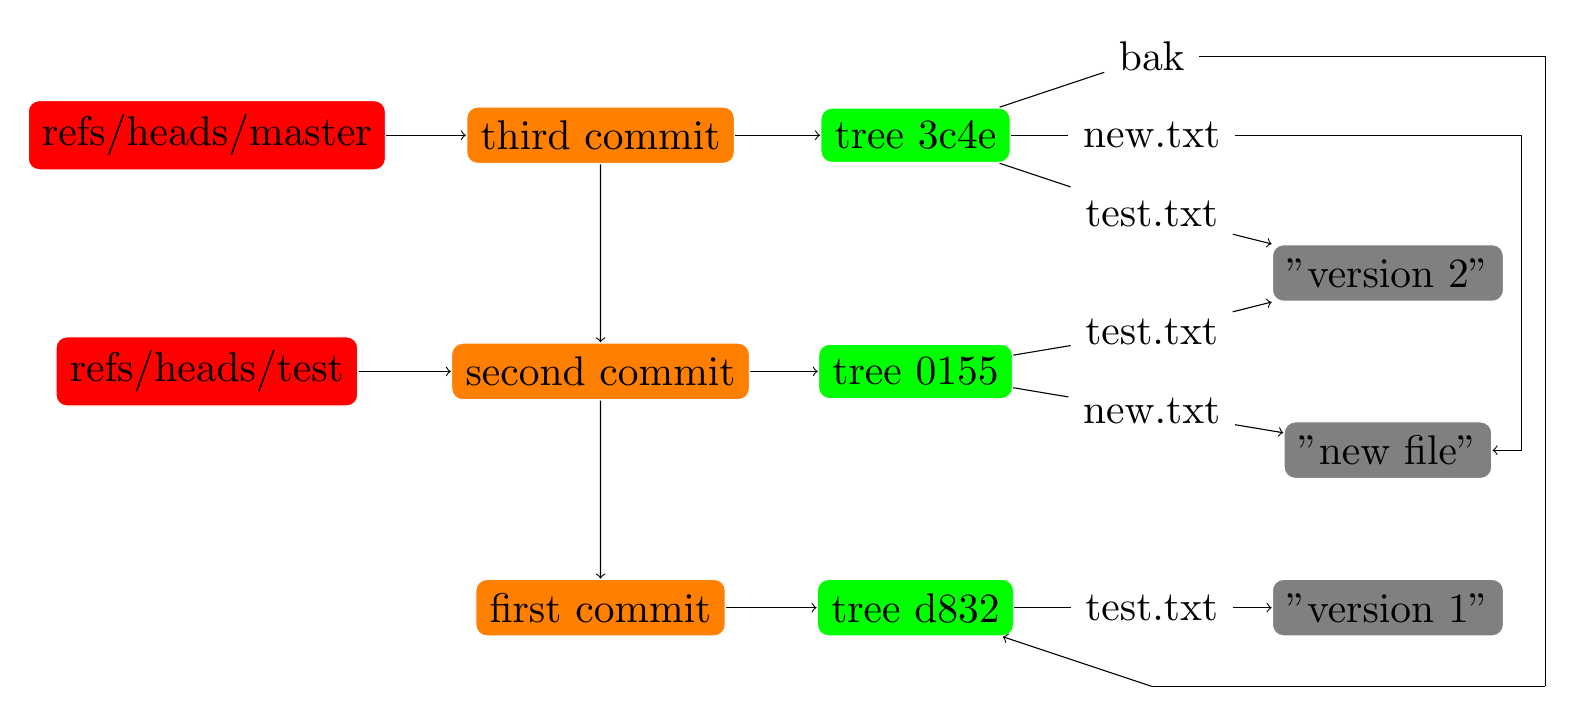
\begin{tikzpicture}
        \node[rectangle,rounded corners, draw=white, fill=red, scale=1.5] (master) at(-5,0){refs/heads/master};
        \node[rectangle,rounded corners, draw=white, fill=red, scale=1.5] (test) at(-5,-3){refs/heads/test};

        \node[rectangle,rounded corners, draw=white, fill=orange, scale=1.5] (3-commit) at(0,0){third commit};
        \node[rectangle,rounded corners, draw=white, fill=orange, scale=1.5] (2-commit) at(0,-3){second commit};
        \node[rectangle,rounded corners, draw=white, fill=orange, scale=1.5] (1-commit) at(0,-6){first commit};
        \draw [->] (master) -- (3-commit);
        \draw [->] (test) -- (2-commit);
        \draw [->] (3-commit) -- (2-commit);
        \draw [->] (2-commit) -- (1-commit);

        \node[rectangle,rounded corners, draw=white, fill=green, scale=1.5] (3-tree) at(4,0){tree 3c4e};
        \draw [->] (3-commit) -- (3-tree);

        \node[rectangle,rounded corners, draw=white, fill=green, scale=1.5] (2-tree) at(4,-3){tree 0155};
        \draw [->] (2-commit) -- (2-tree);

        \node[rectangle,rounded corners, draw=white, fill=green, scale=1.5] (1-tree) at(4,-6){tree d832};
        \draw [->] (1-commit) -- (1-tree);

        \node[rectangle,rounded corners, draw=white, fill=white, scale=1.5] (3-bak) at(7,1){bak};
        \node[rectangle,rounded corners, draw=white, fill=white, scale=1.5] (3-new) at(7,0){new.txt};
        \node[rectangle,rounded corners, draw=white, fill=white, scale=1.5] (3-test) at(7,-1){test.txt};

        \node[rectangle,rounded corners, draw=white, fill=white, scale=1.5] (2-test) at(7,-2.5){test.txt};
        \node[rectangle,rounded corners, draw=white, fill=white, scale=1.5] (2-new) at(7,-3.5){new.txt};

        \node[rectangle,rounded corners, draw=white, fill=white, scale=1.5] (1-test) at(7,-6){test.txt};

        \draw (3-tree) -- (3-bak);
        \draw (3-tree) -- (3-new);
        \draw (3-tree) -- (3-test);

        \draw (2-tree) -- (2-test);
        \draw (2-tree) -- (2-new);

        \draw (1-tree) -- (1-test);

        \node[rectangle,rounded corners, draw=white, fill=gray, scale=1.5] (version-2) at(10,-1.75){"version 2"};
        \node[rectangle,rounded corners, draw=white, fill=gray, scale=1.5] (new-file) at(10,-4){"new file"};
        \node[rectangle,rounded corners, draw=white, fill=gray, scale=1.5] (version-1) at(10,-6){"version 1"};

        \draw [->] (1-test) -- (version-1);
        \draw [->] (2-new) -- (new-file);
        \draw [->] (2-test) -- (version-2);
        \draw [->] (3-test) -- (version-2);
        \draw (3-new) to (11.7, 0);
        \draw [->] (11.7, 0) |- (new-file);
        \draw (3-bak) -| (12, -7);
        \draw (12, -7) -- (7, -7);
        \draw [->] (7, -7) -- (1-tree);

      \end{tikzpicture}
      }
    \end{center}
    \label{fig:reference}
    \caption{Git directory objects with branch head references included}
  \end{figure}
  When you run commands like \code{git branch <branch>},
  Git basically runs update-ref command to add the SHA-1
  of the last commit of the branch you're on into whatever
  new reference you want to create.
  So create branch is just create a reference to some commit.
  And delete branch is only delete a reference.
  After branch deletion, all its objects will be available via their SHAs.
  However, unreachable objects could be deleted via other git operations.
  \item[HEAD] -- Usually the HEAD file is a symbolic reference to the branch
  you're currently on.
  By symbolic reference, we mean that unlike a normal reference,
  it contains a pointer to another reference.\\
  If you look at the file, you'll normally see something like this:\\
  \\
  \code{\$ cat .git/HEAD}\\
  \code{ref: refs/heads/master}\\
  \\If you run \code{git checkout branch}, Git updates the file to look like this:\\
  \\
  \code{\$ cat .git/HEAD}\\
  \code{ref: refs/heads/test}\\

  When you run \code{git commit}, it creates the commit object,
  specifying the parent of that commit object to be whatever SHA-1 value
  the reference in HEAD points to.
  This commit also becomes a new head for a current branch.
  refs/heads/<branch-name> will be updated and map to the SHA
  of this new commit.
  When you do \code{git reset HEAD~1},
  it also only update refs/heads/<branch-name>.
  It takes SHA of parent commit of current head commit.
  \item[Tag (lightweight)] -- It's like a branch reference, but it never moves - it always points to the same commit but gives it a friendlier name.\\
  You can create, update and delete such a tag, and no objects would be affected.
  It's only a reference.
  \item[Tag (annotated)] -- tag object, that points to commit or any other object amd contains metadata, and a reference to this tag object.
\end{description}

\subsubsection{Git file storage internals}

\textbullet\textbf{\large{ loose object storage}}\\

As we mentioned, a git repository take cares of several types of objects:
\code{blob}, \code{tree}, \code{commit}, \code{tag}.
Let's take a look at the details of object storage:\\

git by default writes the objects to directory \code{GIT\_DIR\footnote{the .git directory}/objects}.
Each object is named by a sha1 value, for example \emph{\code{b98191cf971f2418e42877410a6c40fc112a0a93}}\\
it's storage path will be
\begin{center}
\emph{\code{GIT\_DIR/objects/b9/8191cf971f2418e42877410a6c40fc112a0a93}}
\end{center}
the directories under \code{GIT\_DIR/objects} is named by \code{SHA[0,2]} of objects' sha1 value,
this can avoid too much files in one directory because some filesystem has the max link number of files,
such as ext3 has the definition:
\begin{flushleft}
  \code{include/linux/ext3\_fs.h:\#define EXT3\_LINK\_MAX           32000}
\end{flushleft}

One object file is consist of three portions:
\begin{description}
  \item[type] can be one of `blob', `tree', `commit', `tag'
  \item[size] the number of bytes of the content
  \item[content] the content of object
\end{description}

and the object file will be compressed using zlib:

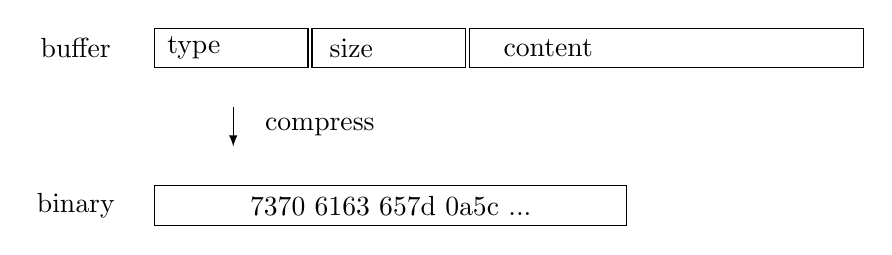
\begin{tikzpicture}
  \node at (0,0.25) {binary};
  \node at (4,0.25) {\code{7370 6163 657d 0a5c ...}};
  \draw (1,0) rectangle (7,0.5);
  \node at (3.1,1.25) {compress};
  \draw[-latex] (2,1.5) -- (2,1);
  \node at (0,2.25) {buffer};
  \node at (1.5,2.25) {type};
  \node at (3.5,2.25) {size};
  \node at (6,2.25) {content};
  \draw (1,2) rectangle (2.95,2.5);
  \draw (3,2) rectangle (4.95,2.5);
  \draw (5,2) rectangle (10,2.5);
\end{tikzpicture}

the compression level can be set by `\textbf{\code{core.compression}}' or `\textbf{\code{core.loosecompression}}'.
\\

\textbullet\textbf{\large{ pack file storage}}\\

When we do \emph{\code{git gc}} or \emph{\code{git repack}}, pack files with the suffix \code{.pack}
maybe be created under directory \emph{\code{GIT\_DIR/objects/pack}}.
A pack is a collection of objects,
individually compressed, with delta compression applied, stored in a single file, with an associated
index file.
Packs are used to reduce the load on mirror systems, backup engines, disk storage, etc.

\begin{lstlisting}[basicstyle=\ttfamily]
$ tree .git/objects/pack
.git/objects/pack
|-- pack-24fcb83682e5a2848ef7bd00a9eda0bff1a372fc.idx
|-- pack-24fcb83682e5a2848ef7bd00a9eda0bff1a372fc.pack
|-- pack-915d8b4ae03b03179912c589cee932e5a990b7f0.idx
|-- pack-915d8b4ae03b03179912c589cee932e5a990b7f0.pack
|-- ...
\end{lstlisting}

Conceptually there are only four object types in a pack file: commit, tree, tag and blob.
However to save space, an object could be stored as a ``delta'' of another ``base'' object.
These representations are assigned new types \code{ofs-delta} and \code{ref-delta}.

\begin{description}
  \item[delta object]
    Both ofs-delta and ref-delta store the ``delta'' to be applied to another object
    (called `base object') to reconstruct the object. The difference between them is,
    ref-delta directly encodes 20-byte base object name. If the base object is in the same pack,
    ofs-delta encodes the offset of the base object in the pack instead.
  \item[base object]
    The base object could also be deltified if it's in the same pack.
    Ref-delta can also refer to an object outside the pack. When stored on disk however,
    the pack should be self contained to avoid cyclic dependency.
\end{description}

And usualy we have lots of versions of a single file in a repository, a new pack file will
store the last version's content as the base object, and computes the earlier versioins to
to be delta objects and store them referring to the base object:

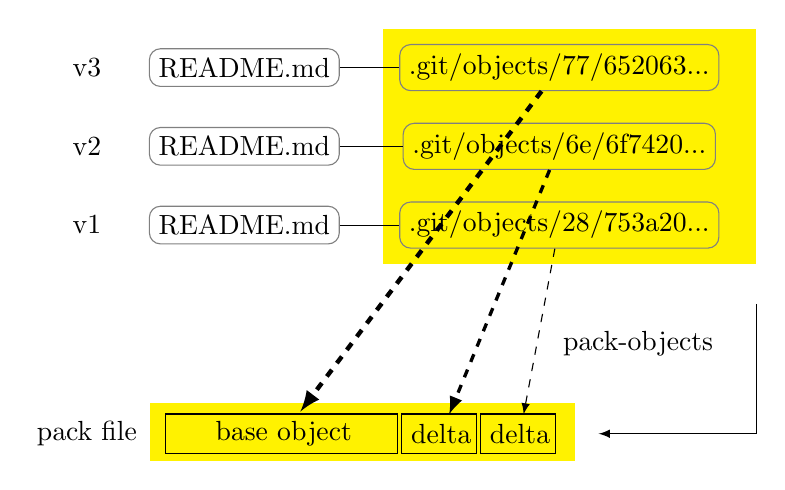
\begin{tikzpicture}
  % loose objects
  \filldraw[fill=yellow, draw=white] (3.75,2.5) rectangle (8.5,5.5);

  \node at(0,5){v3};
  \node[rectangle,rounded corners, draw=gray,] (v3) at(2,5){README.md};
  \node[rectangle,rounded corners, draw=gray,] (v3obj) at(6,5){.git/objects/77/652063...};
  \node at(0,4){v2};
  \node[rectangle,rounded corners, draw=gray,] (v2) at(2,4){README.md};
  \node[rectangle,rounded corners, draw=gray,] (v2obj) at(6,4){.git/objects/6e/6f7420...};
  \node at(0,3){v1};
  \node[rectangle,rounded corners, draw=gray,] (v1) at(2,3){README.md};
  \node[rectangle,rounded corners, draw=gray,] (v1obj) at(6,3){.git/objects/28/753a20...};
  \draw (v3) -- (v3obj);
  \draw (v2) -- (v2obj);
  \draw (v1) -- (v1obj);

  % arrow
  \draw (8.5,2) -- (8.5,0.35);
  \draw[-latex] (8.5,0.35) -- (6.5,0.35);
  \node at(7,1.5){pack-objects};

  % pack file
  \filldraw[fill=yellow, draw=white] (0.8,0) rectangle (6.2,0.75);
  \node at (0,0.35) {pack file};
  \node (base) at (2.5,0.35) {base object};
  \node (deltav2) at (4.5,0.35) {delta};
  \node (deltav1) at (5.5,0.35) {delta};
  \draw (1,0.1) rectangle (3.95,0.6);
  \draw (4,0.1) rectangle (4.95,0.6);
  \draw (5,0.1) rectangle (5.95,0.6);

  \draw[dashed, ultra thick, -latex] (v3obj) -- (base);
  \draw[dashed, very thick, -latex] (v2obj) -- (deltav2);
  \draw[dashed, -latex] (v1obj) -- (deltav1);
\end{tikzpicture}

Usually objects contained in the pack are compressed using zlib, the compression level
can be set by `\textbf{\code{core.compression}}' or `\textbf{\code{pack.compression}}'.

When objects contained in the pack are stored using delta compression. The objects
are first internally sorted by type, size and optionally names and compared against
the other objects to see if using delta compression saves space. `\textbf{\code{pack.depth}}'
limits the maximum delta depth; Making it too deep affects the performance on the unpacker side,
because delta data needs to be applied that many times to get to the necessary object.
\\

To quickly find objects in the pack file, an associated index file is created with the
\emph{\href{https://github.com/git/git/blob/master/Documentation/technical/pack-format.txt\#L161}{format}},
And `\emph{\code{git index-pack}}' can be used to regenerate the *.idx file on the *.pack file.
\\

\textbullet\textbf{\large{ when pack file is created}}\\

When we talk about the pack files, we said that packs are used to reduce the load on mirror systems,
backup engines, disk storage, etc. So pack files will created in several scenes:

\begin{description}
  \item[git gc] `\emph{\code{git gc}}' runs a number of housekeeping tasks within the repository,
    such as compressing file revisions (to reduce disk space and increase performance), removing
    unreachable objects which may have been created from prior git commands.
    We can run it manually, and it may create a new pack file.
  \item[git repack] `\emph{\code{git repack}}' is used to combine all objects that do not currently
    reside in a pack file into a pack. It can also be used to re-organize existing packs into
    a single, more efficient pack.
  \item[git push] `\emph{\code{git push}}' will run \code{send-pack} to connects to the remote side,
    it gets one file descriptor which is either a socket (over the network) or a pipe (local).
    What's written to this file descriptor goes to `\emph{\code{git-receive-pack}}' to be unpacked.
    We can get the following pipeline flow from\\
    \emph{\href{https://github.com/git/git/blob/master/Documentation/technical/send-pack-pipeline.txt}{Documentation/technical/send-pack-pipeline.txt}}:
    \begin{lstlisting}[basicstyle=\ttfamily]
    send-pack
       |
       pack_objects() --> fd --> receive-pack
          | ^ (pipe)
          v |
       (child)
    \end{lstlisting}
    so we can see that `\emph{\code{git push}}' will create a pack file and send it to the remote side.
  \item[git-receive-pack] As menthioned above, `\emph{\code{git-receive-pack}}' will receive a pack file
    from `\emph{\code{git push}}'. And `\emph{\code{git receive-pack}}' will also forked a child
    `\emph{\code{git gc --auto --quiet}}' to check if there are too many loose objects to pack.
    Ususaly the threshold is 6700 loose files, we can set it by `\textbf{\code{gc.auto}}'.
  \item[git-upload-pack] When clients runs `\emph{\code{git clone}}' or `\emph{\code{git fetch}}', the
    client connects to the remote side and invokes `\emph{\code{git-upload-pack}}'.
    `\emph{\code{git-upload-pack}}' will communicate with client and compute how many objects the client
    want then fork and exec child `\emph{\code{git-pack-objects}}' to create a pack file for all the
    needed objects and pipe the pack file to client.
    \begin{lstlisting}[basicstyle=\ttfamily]
    upload-pack
       |
       pack_objects() --> fd --> fetch-pack
          | ^ (pipe)
          v |
       (child)
    \end{lstlisting}

    We can also use the `\textbf{\code{repack.writeBitmaps}}' to let git write a bitmap index when packing
    all objects to disk (e.g., when git repack -a is run). This index can speed up the "counting
    objects" phase of subsequent packs created for clones and fetches, at the cost of some disk space
    and extra time spent on the initial repack.

\end{description}
